%%%%%%%%%%%%%%%%%%%%%%%%%%%%%%%%%%%%%%%%%%%%%%%%%%
%%%%%%%%%%%%%%%%%%%%%%%%%%%%%%%%%%%%%%%%%%%%%%%%%%
%%
%% Based one the "beamer-greek-two" template provided 
%% by the Laboratory of Computational Mathematics, 
%% Mathematical Software and Digital Typography, 
%% Department of Mathematics, University of the Aegean
%% (http://myria.math.aegean.gr/labs/dt/)
%%
%% Adapted by John Liaperdos, October-November 2014
%% (ioannis.liaperdos@gmail.com)
%%
%% Last update: 22/06/2017 (English Support)
%%
%%%%%%%%%%%%%%%%%%%%%%%%%%%%%%%%%%%%%%%%%%%%%%%%%%
%%%%%%%%%%%%%%%%%%%%%%%%%%%%%%%%%%%%%%%%%%%%%%%%%%
%%
\PassOptionsToPackage{unicode}{hyperref}
\PassOptionsToPackage{naturalnames}{hyperref}
\documentclass{beamer} 
%\usepackage{babel}
%\usepackage[utf8]{inputenc}
\usepackage[longnamesfirst,square,numbers,comma,sort&compress]{natbib}
\usepackage{graphicx}
\usepackage{todonotes}
\usepackage[flushleft]{threeparttable}
% \usepackage{multirow}
% \usepackage{nameref}
% \usepackage{amsmath}
\usepackage{wrapfig}

%%% FONT SELECTION %%%%%%%%%%%%%%%%%
%%% we choose a sans font %%%%%%%%%%
\usepackage{kmath,kerkis} 
%\usepackage[default]{gfsneohellenic} 
%%%%%%%%%%%%%%%%%%%%%%%%%%%%%%%%%%%%

\usepackage{color}
\usepackage{amsmath}
\usepackage{amssymb}
\usepackage{media9}

\usepackage{epstopdf}
\usepackage{graphicx}
\graphicspath{{./images/}}

%%
% load TEI-Pel - specific layout
\usepackage{TeiPel_En_Beamer_Layout}
\setTeipelLayout{newlogo}% options: "draft", "newlogo"

%%%%%%%%%%%%%%%%%%%%%%%%%%%%%%%%%%%%%%%%%%%%%%%%%%%%%%%%%%%%
% Thesis Info %%%%%%%%%%%%%%%%%%%%%%%%%%%%%%%%%%%%%%%%%%%%%%
%%%%%%%%%%%%%%%%%%%%%%%%%%%%%%%%%%%%%%%%%%%%%%%%%%%%%%%%%%%%
	% title
		\title[Thesis]{Comprehensive machine-learning-based analysis of microRNA-target interactions reveals variable transferability of interaction rules across species}	
	% author 
    % (In the mandatory argument "{}", separate multiple
    % authors with "\and" - use "\\" for better author name formatting
    % in the title page. In the optional argument "[]" include all
	% author names, with no "\and" or text formatting macros.)
	% Example: 
    %\author[A. Author Albert Einstein]{Anthony Author \and Albert Einstein}
		\author[A. Author]{Gilad Ben Or}
	% supervisor	
		\supervisor{Supervisor}{Isana Veksler-Lublinsky}{PhD}
	% date
		\presentationDate{October 28, 2020}
%%%%%%%%%%%%%%%%

\begin{document}

% typeset front slides
	\typesetFrontSlides

%%%%%%%%%%%%%%%%
% Your Slides Start here:

%%%%
\section{Background}

%%
\subsection[Background]{MicroRNA background}

\begin{frame}{The Central Dogma of Molecular Biology}
	\begin{exampleblock}
		<1->{}
		\begin{itemize}
			\item Published by Francis Crick in 1957-1958
			\item "DNA makes RNA, and RNA makes protein"
		\end{itemize}
	\end{exampleblock}
	\begin{figure}[ht!]
		\centering
		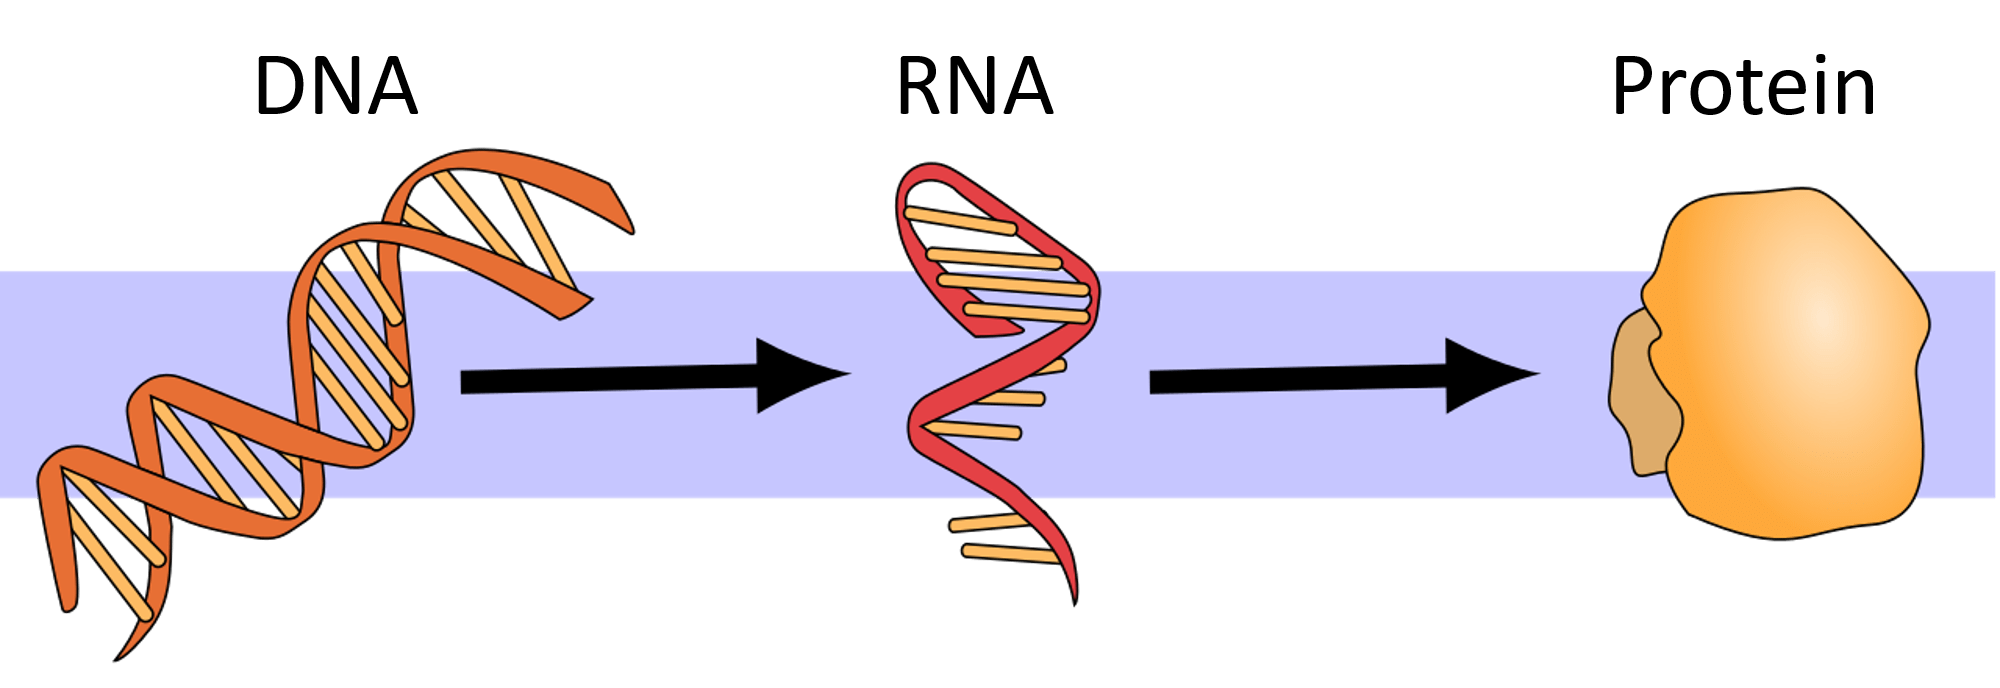
\includegraphics[width=0.8\textwidth]{images/dogma.png}
	\end{figure}
\end{frame}

\begin{frame}{Regulation of Gene Expression}
	\begin{exampleblock}
		<1->{}
		\begin{itemize}
			\item Mechanisms that are used by cells to increase or decrease the production of specific gene products (protein or RNA)
		\end{itemize}
	\end{exampleblock}
	\begin{figure}[ht!]
		\centering
		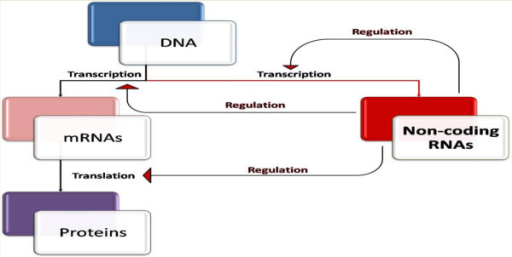
\includegraphics[width=0.8\textwidth]{images/modifieddogma.png}
	\end{figure}
\end{frame}



\begin{frame}{MicroRNA}
	\begin{exampleblock}
		<1->{}
		\begin{itemize}
			\item A class of small non-coding RNAs (19-24 nts)\\
			      \textbf{hsa-miR-1: UGGAAUGUAAAGAAGUAUGUAU
			      	}\item Regulate gene expression by binding to partially complementary sites
			      on target mRNAs (hybridization)
		\end{itemize}
	\end{exampleblock}
% 	\begin{itemize}
% 		% \item MicroRNAs (miRNAs) are small non-coding RNAs that regulate gene expression post-transcriptionally. 
% 		% \item Mature miRNAs form the core of the miRNA-induced silencing complex with Argonaute proteins (miRISC).
% 		% \item miRISC uses the sequence information in the miRNA as a guide to recognize and bind with target mRNAs.
% 	\end{itemize}
	\begin{figure}[ht!]
		\centering
			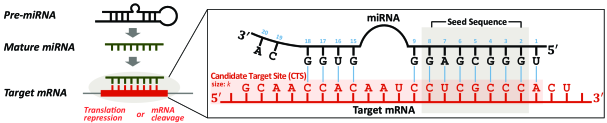
\includegraphics[width=0.8\textwidth]{images/mirna-target.png}
		\end{figure}
\end{frame}


\begin{frame}{MicroRNA}
	\begin{itemize}
% \item miRISC binding typically leads to translational inhibition and/or degradation of targeted mRNAs.
\item Lead to translational inhibition and/or degradation of targeted mRNAs
\item Conserved throughout evolution
\item Present in the genomes of animals and plants  
\item Have diverse functions in development and physiology
\item Have been implicated in many human diseases
\end{itemize}
	\begin{exampleblock}
		<1->{}
		\begin{itemize}
			\item Found in all mammalian cells
			\item Unique to cell type
			\item Unique to cell states
		\end{itemize}
	\end{exampleblock}

\end{frame}

\subsection{Identification of miRNA target sites}
%%%%%%%%%%%%%%%%%%%%%%%%%%%%%%%%%%
\begin{frame}{Identification of miRNA target sites}
\begin{exampleblock}
		<1->{}
		The identification of miRNA target sites on mRNAs is a fundamental step in understanding miRNA involvement in cellular processes.
	\end{exampleblock}
	\begin{itemize}
	\item Laboratory experiments
	\item Bionformatics methods
\end{itemize}
\begin{figure}[ht!]
	  \centering
    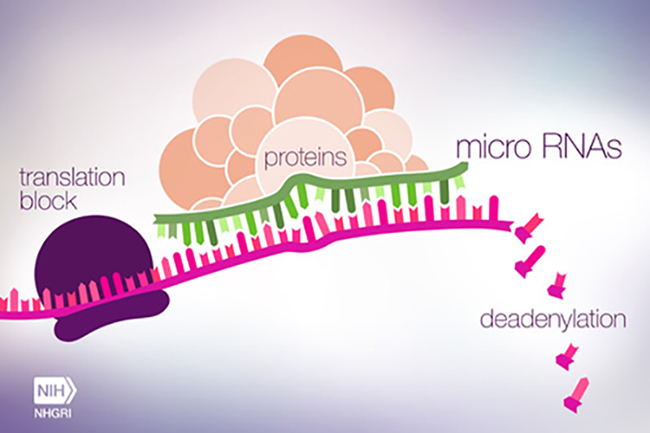
\includegraphics[width=0.5\textwidth]{images/micro_rna2910516058.jpg} 
\end{figure}
\end{frame}



\begin{frame}{Experimental methods}
	\begin{column}{0.65\textwidth}
		\begin{exampleblock}
			<1->{Measuring changes in mRNA levels}
			Measuring level changes in tissue-cultured cells.
			\begin{itemize}
				\item Cons: indirect signals, exact sequences are unknown, may miss signals.
			\end{itemize}
		\end{exampleblock}
		\begin{exampleblock}
			<1->{Crosslinking and immunoprecipitation (CLIP)}
			CLIP of RNA-protein complexes that are found in direct contact.
			\begin{itemize}
				\item Cons: the identity of the specific miRNA has to be predicted bioinformatically.
			\end{itemize}
		\end{exampleblock}
	\end{column}
	\begin{column}{0.35\textwidth}
		\begin{figure}[hb!]
			\centering
			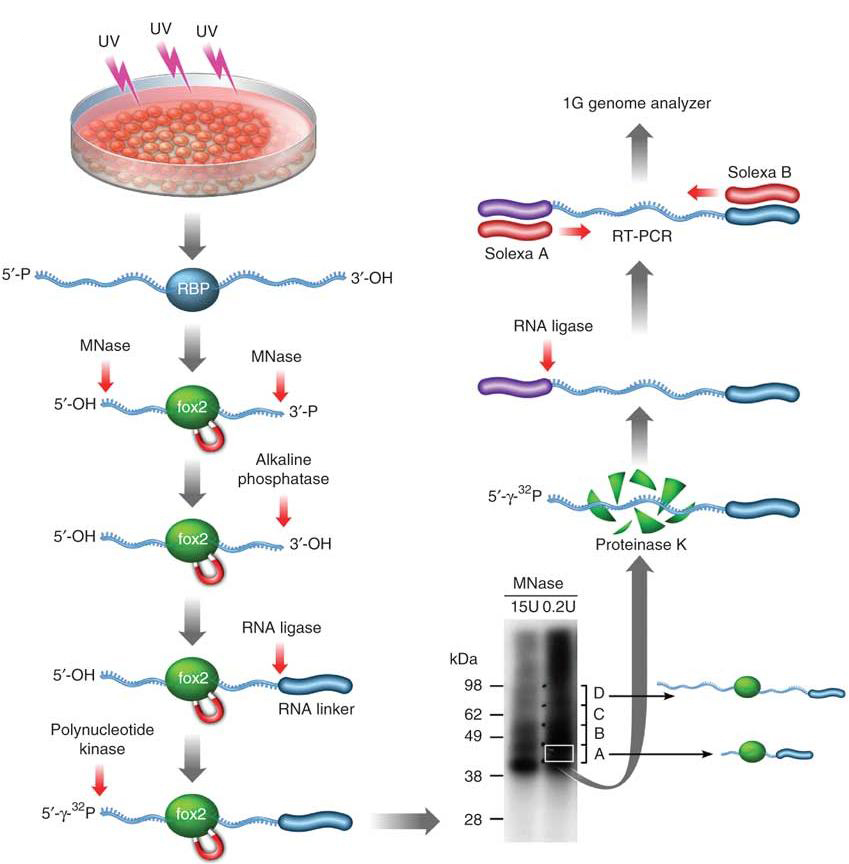
\includegraphics[width=0.8\textwidth]{images/Crosslinking-and-Immunoprecipitation-(CLIP)-2.jpg}
		\end{figure}
	\end{column}
\end{frame}


\begin{frame}{Experimental methods}
\begin{exampleblock}
		<1->{Advanced methods}
		  capture miRNAs bound to their respective targets
	\begin{itemize}
\item CLASH (Cross-linking, Ligation and Sequencing of Hybrids)
\item CLEAR (covalent ligation of endogenous Argonaute-bound RNAs)-CLIP 
\item Modified iPAR-CLIP 
\end{itemize}
\end{exampleblock}
These methdos use an extra step to covalently ligate the 3' end of a miRNA and the 5' end of the associated target RNA within the miRISC. 
\end{frame}

\begin{frame}{Experimental methods}
\begin{figure}[hb!]
	  \centering
% 	  \caption{Crosslinking and immunoprecipitation (CLIP)}
    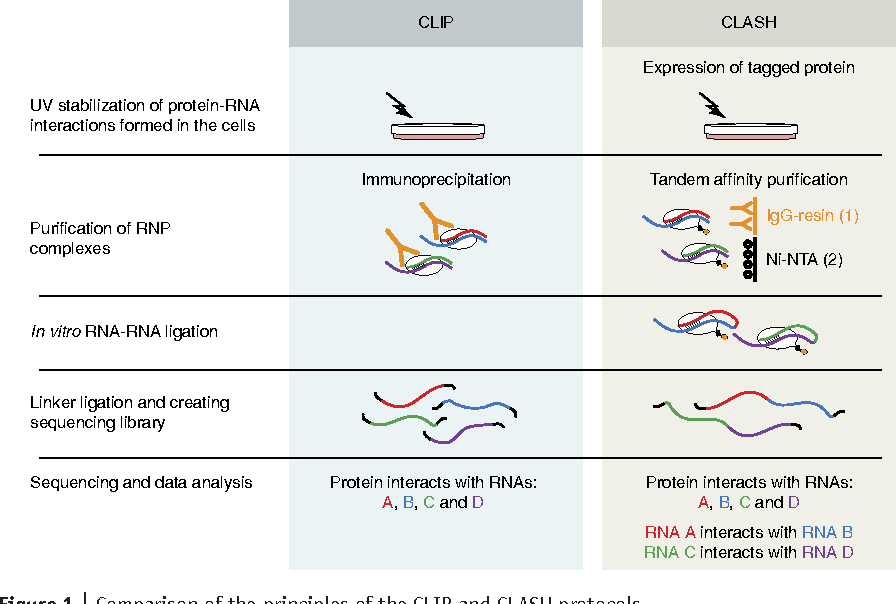
\includegraphics[width=0.8\textwidth]{images/clash11.png}
\end{figure}
\end{frame}


\begin{frame}{Principles of Bioinformatics methods}
\begin{itemize}
\item Base pairing pattern (e.g., seed)
\item Free energy of the miRNA-mRNA duplex
\item Evolutionarily conservation of the target gene
\item Accessibility of the mRNA (mRNA secondary structure)
\end{itemize}
\begin{figure}[hb!]
	  \centering
% 	  \caption{Crosslinking and immunoprecipitation (CLIP)}
    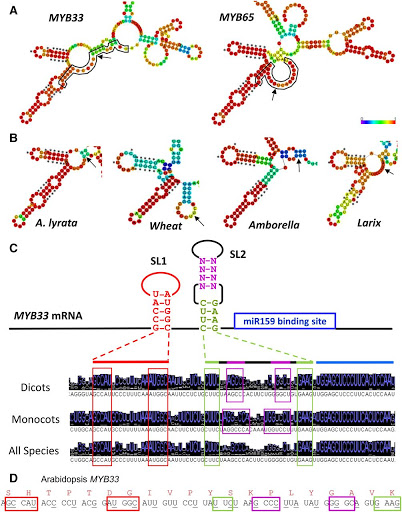
\includegraphics[width=0.4\textwidth]{images/mirna seed second.jpg}
\end{figure}
\end{frame}

%%%%%%%%%%%%%%%%%%%%%%%%%%%%%%%%%%%%%%%%%%%%%%%%%%%%%%%%%%%%%%%%%%%%%%%%%%%%%
%%%%%%%%%%%%%%%%%%%%%%%%%%%%%%%%%%%%%%%%%%%%%%%%%%%%%%%%%%%%%%%%%%%%%%%%%%%
\section{Motivaton}

\subsection{Previous work}
%%%%%%%%%%%%%%%%%%%%%%%%%%%%%%%%%%%%%%


\begin{frame}{Avaliable datasets}
% 	\begin{itemize}
% 	\item Direct experiments
% 		\begin{itemize}

% 	\item Human - 2 
% 	\item \textit{Caenorhabditis elegans (C. elegans)} - 2
% 	\item Cattle \textit{Bos taurus} -1
% 	\item Mouse - 1
% 	\end{itemize}
% 	\pause
% 		\item re-analysis of previous experiments
% 			\begin{itemize}
% \item Human - 1
% \item Mouse - 1
% 		\end{itemize}
% 	\end{itemize}

\begin{table}[h!]
\label{tbl:dataset_description}
% \begin{tabular}{ | l | l | l | l | l | }
 \resizebox{\textwidth}{!}{%
\begin{tabular}{|l|p{5cm}|p{4cm}|c|}
	\hline
	\textbf{Name} & \textbf{Cell/ Developmental stage} & \textbf{Experimental Method} & \textbf{Organism} \\
	\hline
	
% 	cattle\_MDBK & 
    ca1 &
	Madin-Darby bovine kidney (MDBK) &
	CLEAR-CLIP  &                      
	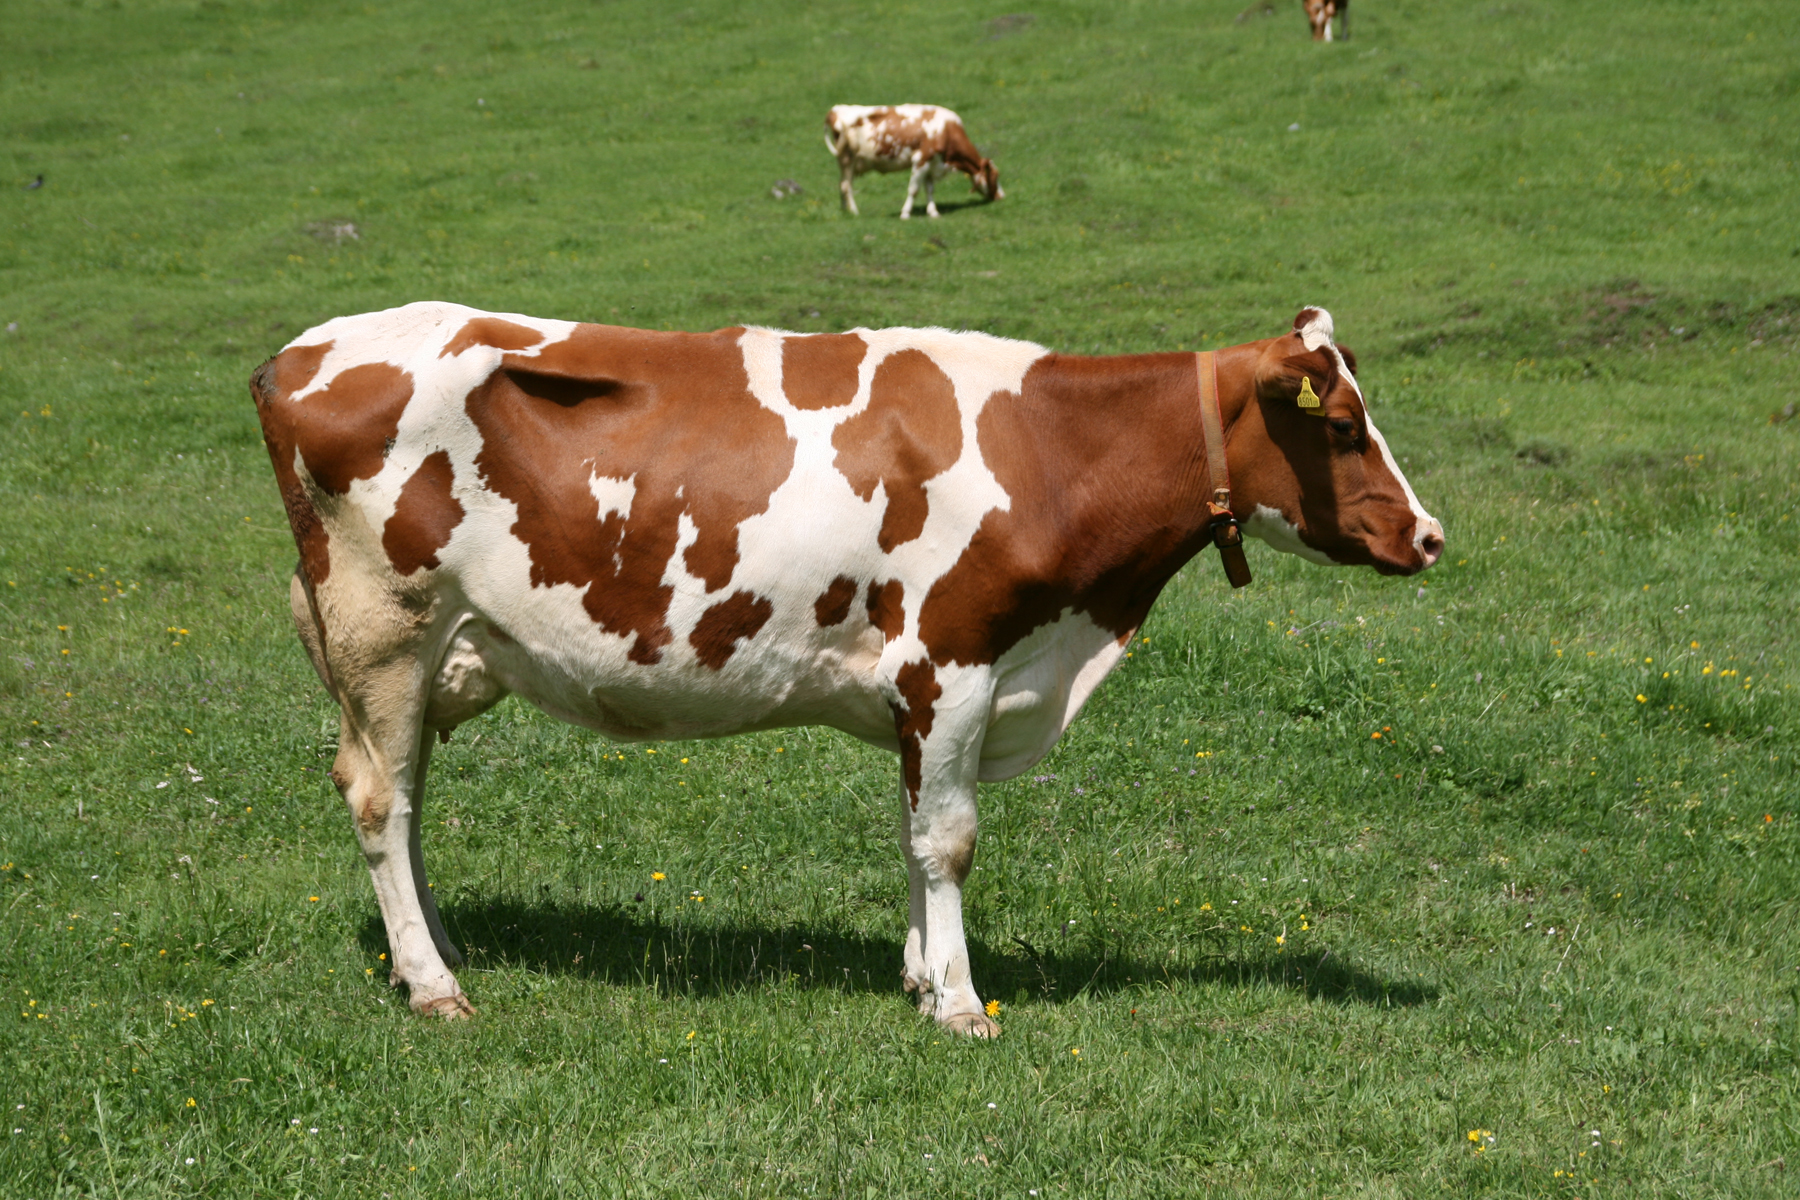
\includegraphics[height=0.4cm]{images/Bos_taurus_taurus_sideview.jpg} \\
	\hline
% 	celegans\_L3 & 
    ce1 &
	L3 staged & 
	Modified iPAR-CLIP & 
	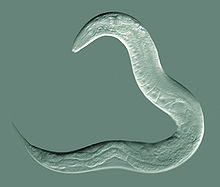
\includegraphics[height=0.4cm]{images/220px-CelegansGoldsteinLabUNC.jpg} \\
	\hline
% 	celegans\_L4 & 
    ce2 &
	Mid-L4 WT (N2)  & 
	ALG-1 iCLIP endogenous ligation & 
	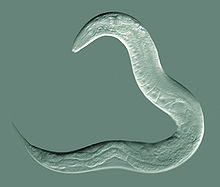
\includegraphics[height=0.4cm]{images/220px-CelegansGoldsteinLabUNC.jpg} \\
	\hline
% 	human\_HEK293 & 
    \textbf{h1} &
	\textbf{Human embryonic kidney293 cells (HEK293)} & 
	\textbf{CLASH}  & 
	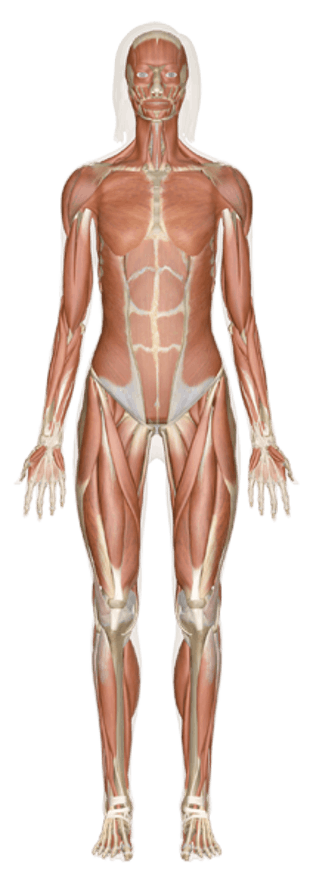
\includegraphics[height=0.4cm]{images/human.png} \\
	\hline
	
% 	human\_mix & 
    h2 &
	A mix of 6 datasets & 
	AGO-CLIP endogenous ligation &  
	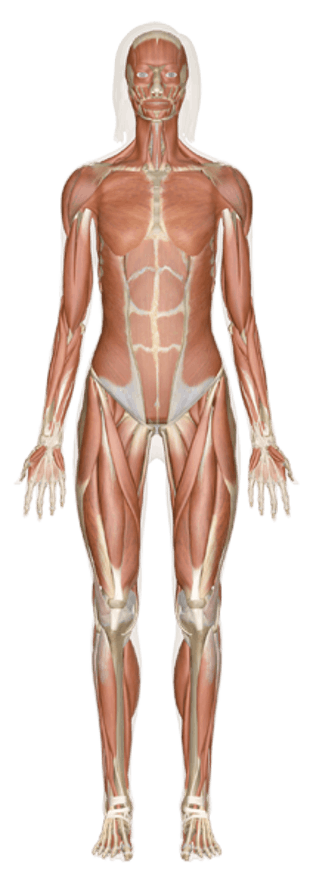
\includegraphics[height=0.4cm]{images/human.png} \\
	\hline
	
% 	human\_huh7.5 & 
    h3 &
	Human hepatoma cells (Huh-7.5) & 
	CLEAR-CLIP & 
	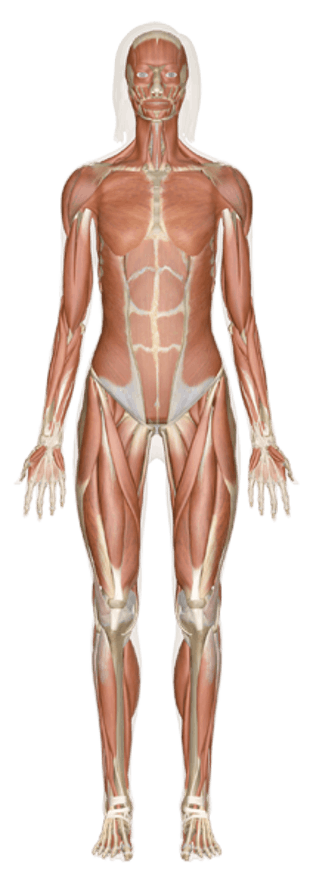
\includegraphics[height=0.4cm]{images/human.png} \\
	\hline
	
% 	mouse\_mix & 
    m1 &
	A mix of 3 datasets & 
	AGO-CLIP endogenous ligation & 
	 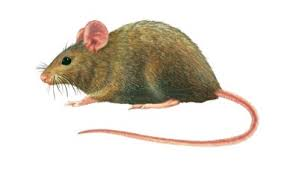
\includegraphics[height=0.4cm]{images/mosmus.jpg} \\
	\hline
	
% 	mouse\_ATCC & 
    m2 &
	N2A mouse neuroblastoma (ATCC) & 
	CLEAR-CLIP & 
	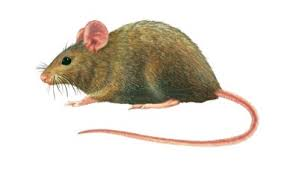
\includegraphics[height=0.4cm]{images/mosmus.jpg} \\
	\hline
\end{tabular}}
\end{table}


\end{frame}



\begin{frame}{Previous work}
\begin{column}{0.65\textwidth}
Target prediction algorithms can be grouped into three categories:
\begin{itemize}
\item ab initio 
\item machine learning 
\item hybrid approaches
\end{itemize}
\end{column}
\begin{column}{0.35\textwidth}
\begin{figure}[hb!]
	  \centering
% 	  \caption{Crosslinking and immunoprecipitation (CLIP)}
    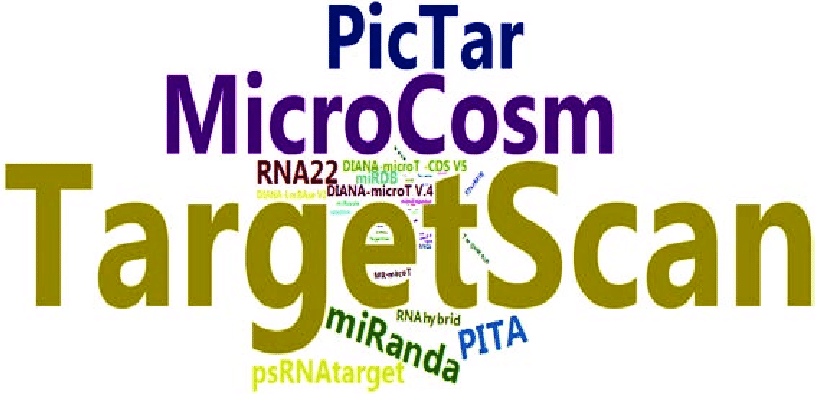
\includegraphics[width=\textwidth]{images/Word-cloud-for-relative-use-of-miRNA-target-prediction-tools-based-on-number-of.png}
\end{figure}
\end{column}
\begin{exampleblock}
		<1->{Machine learning algorithms}
The methods differ in several aspects:	
\begin{itemize}
\item ML approach
\item Features
\item Datasets for training and testing
\item Generation of negative data
\end{itemize}
\end{exampleblock}


% Several ML-based methods utilized chimeric miRNA-target datasets to build and evaluate models. These methods differ in several aspects:
% \begin{enumerate}
% \item ML approach
% \item Features
% \item Datasets for training and testing
% \item Generation of negative data
% \end{enumerate}

\end{frame}


\begin{frame}{Previous work}

\begin{table}[h!]
\centering

\caption{A summary of machine-learning based methods that utilized chimeric miRNA-target datasets in their models.}
\label{tab:toolsummary}
\centering
   \resizebox{\textwidth}{!}{%

\begin{tabular}{|l|l|l|l|l|l|}
\hline
\textbf{Tool} & \textbf{ML method} & \textbf{Datasets used for training/testing}                                     & \textbf{Independent Dataset}                                                   & \textbf{Negative interactions} & \textbf{Features} \\ \hline
chimiRic \cite{lu2016learning}      & SVM                & Human (CLASH, AGO-CLIP)                                                                                            & \begin{tabular}[c]{@{}l@{}} chimeras from \\ Mouse and \textit{C.elegans} \end{tabular}                                                              & \begin{tabular}[c]{@{}l@{}}seed matching \\ non-CLIP sites \end{tabular}                   & Small             \\ \hline
TarPmiR \cite{ding2016tarpmir}       & Random Forest      & Human (CLASH)                                                                                                         & \begin{tabular}[c]{@{}l@{}}Human (PAR-CLIP), \\ Mouse (HITS-CLIP)\end{tabular}   & \begin{tabular}[c]{@{}l@{}}Negative target sites, \\ on positive mRNAs\end{tabular}                     & 13                \\ \hline
DeepMirTar \cite{wen2018deepmirtar}   & Deep learning      & Human (CLASH) + mirRecords                                                                                            & Human (PAR-CLIP)                                                                & Mock miRNAs                          & 750               \\ \hline
miRAW \cite{pla2018miraw}        & Deep learning      & \begin{tabular}[c]{@{}l@{}}Human (intersection of: CLASH, CLIP, \\ TargetScan with Diana TarBase, mirTarBase)\end{tabular} & Human (microarray)                                                              & Experimental data                  & Raw sequence       \\ \hline
mirLSTM \cite{paker2019mirlstm}      & Deep learning      & Human (CLASH) + mirRecords                                                                                            & Experimental                                                                   & Mock miRNAs                          & Raw sequence       \\ \hline
mirTarget \cite{wang2016improving}    & SVM                & Human (CLASH, AGO-CLIP)                                                                                               & Human(microarrays)                                                              & \begin{tabular}[c]{@{}l@{}}seed matching non-CLIP sites \\ on expressed mRNAs \end{tabular}                           & 50                \\ \hline
mirTarget v4 \cite{liu2019prediction} & SVM                & \begin{tabular}[c]{@{}l@{}}Human (Intersection of \\ CLASH and microarrays) \end{tabular}                                                                                             & \begin{tabular}[c]{@{}l@{}}Mouse (HITS-CLIP), \\ Human (microarrays)\end{tabular} & \begin{tabular}[c]{@{}l@{}}seed matching non-CLIP sites \\ on expressed mRNAs \end{tabular}                          & 96                \\ \hline
\end{tabular}}
\end{table}
\end{frame}


\begin{frame}{DeepMirTar}
\begin{itemize}
\item DeepMirTar is based on a stacked de-noising auto-encoder deep learning method (SdA).
\item Uses 750 different features to describe the interactions.
\end{itemize}
\begin{column}{0.5\textwidth}
\begin{exampleblock}
		<1->{Features}
seed match, sequence composition, free energy, site accessibility, conservation, and hot-encoding of miRNAs and their target sites
\end{exampleblock}
\end{column}
\begin{column}{0.5\textwidth}
\begin{figure}[]
	  \centering
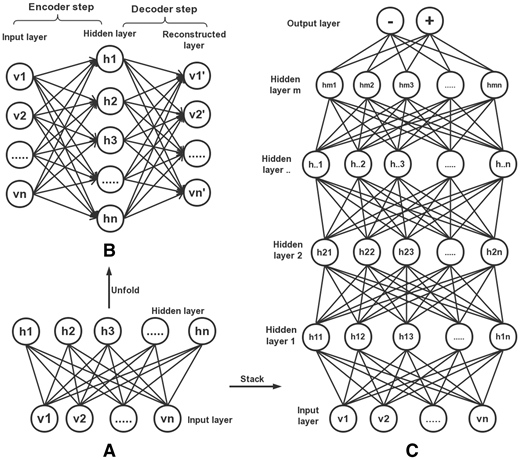
\includegraphics[width=0.8\textwidth,keepaspectratio]{images/deepmirtarsda.png}
\end{figure}
\end{column}
\end{frame}

\begin{frame}{Accuracy performance}
\begin{table}[h!]
\caption{taken from deepMirTar \cite{wen2018deepmirtar}.}
\label{tab:existingmethods}
\centering
   \resizebox{\textwidth}{!}{%

\begin{tabular}{lll|l|l|}
\cline{1-2} \cline{4-5}
\multicolumn{1}{|l|}{\textbf{Methods}} & \multicolumn{1}{l|}{\textbf{ACC}} & \textbf{} & \textbf{Machine learning alg.} & \textbf{ACC}    \\ \cline{1-2} \cline{4-5} 
\multicolumn{1}{|l|}{Miranda}          & \multicolumn{1}{l|}{0.6592}       &           & DT (Decision Tree)                            & 0.8139 (0.0137) \\ \cline{1-2} \cline{4-5} 
\multicolumn{1}{|l|}{RNAhybrid}        & \multicolumn{1}{l|}{0.6988}       &           & BNB (Bernoulli Naïve Bayes)                            & 0.7570 (0.0098) \\ \cline{1-2} \cline{4-5} 
\multicolumn{1}{|l|}{PITA}             & \multicolumn{1}{l|}{0.4981}       &           & LR (Logistic Regression)                            & 0.8491 (0.0117) \\ \cline{1-2} \cline{4-5} 
\multicolumn{1}{|l|}{TargetScan v7.0a} & \multicolumn{1}{l|}{0.5801}       &           & RF (Random Forest)                             & 0.8811 (0.0090) \\ \cline{1-2} \cline{4-5} 
\multicolumn{1}{|l|}{TarPmiR}          & \multicolumn{1}{l|}{0.7446}       &           & MLP (Multi-Layer Perceptron)                            & 0.8990 (0.0099) \\ \cline{1-2} \cline{4-5} 
\multicolumn{1}{|l|}{\textbf{DeepMirTar (SdA)}} & \multicolumn{1}{l|}{0.9348}       &           & CNN-1D (Convolutional Neural Network)                         & 0.8886 (0.0145) \\ \cline{1-2} \cline{4-5} 
                                       &                                   &           & CNN-2D (Convolutional Neural Network)                         & 0.8765 (0.0169) \\ \cline{4-5} 
\end{tabular}}
\end{table}
\end{frame}



\subsection{Research Questions}
%%%%%%%%%%%%%%%%%%%%%%%%%%%%%%%%%%

\begin{frame}{Research Questions}
	\begin{itemize}

\item We would like to study the transferability of miRNA-target interaction rules between organisms
\begin{enumerate}
% \item What are the available datasets of chimeric miRNA-target interactions from a variety of organisms?
\item \textbf{Normalization} - What are the specifications of a standard format, to represent all the available datasets?
\pause
\item \textbf{Features} - What are the high-level and raw-level features that best represent interactions?
\pause
\item \textbf{Top important features} - What are the key features of miRNA-target interactions for each organism?
\pause
\item \textbf{Inter-organism  performance} - What is the performance of machine learning models in predicting organism interactions different from the one they have trained on?
\pause
\item \textbf{Model transferability} - What are the different factors that best explain the observed results, and do they coincide with the evolutionary distance?
\end{enumerate}

	\end{itemize}
\end{frame}



% \begin{frame}{Research Questions}
% % \textbf{We would like to study the transferability of miRNA-target interaction rules between organisms
% % }
% \begin{exampleblock}
% 		<1->{Dataset standard format}
% What are the specifications of a standard format, to represent all the available datasets?
% \end{exampleblock}
% \pause
% \begin{exampleblock}
% 		<1->{Features}
% What are the high-level and raw-level features that best represent interactions?
% \end{exampleblock}
% \pause
% \begin{exampleblock}
% 		<1->{Top important features}
% What are the key features of miRNA-target interactions for each organism?\end{exampleblock}
% \pause
% \begin{exampleblock}
% 		<1->{Inter-organism prediction performance}
% What is the performance of machine learning models in predicting organism interactions different from the one they have trained on?
% \end{exampleblock}
% \pause
% \begin{exampleblock}
% 		<1->{model transferability}
% What are the different factors that best explain the observed results, and do they coincide with the evolutionary distance?
% \end{exampleblock}


% % \item What is the performance of machine learning models in predicting organism interactions different from the one they have trained on?
% % \item What are the different factors that best explain the observed results, and do they coincide with the evolutionary distance?
% % \end{enumerate}

% % 	\end{itemize}
% \end{frame}



\section{Methods \& Results}
%%%%%%%%%%%%%%%%%%%%%%%%%%%%%%%%%%%%%%%%%%%%%%%%%%%%%%%%
\subsection{Processing pipeline}
\begin{frame}{Processing pipeline}
\begin{itemize}
\item Transform and unify the datasets' different data formats.
\begin{enumerate}
\item Retrieve missing miRNA sequences (\textbf{miRBase}).
\item Extract target sequences based on the \textbf{genomic coordinates}. 
\item \textbf{BLAST}  to match the target mRNA sequences against the \textbf{3'UTRs} (Ensembl Biomart).
\item \textbf{Duplex generation} using ViennaRNA suite (RNAduplex).
\item Keeping \textbf{canonical and non-canonical} seed interactions only.
\end{enumerate}
% \item Enable, with a relatively low effort, to add more data sources to the analysis.
\end{itemize}



\begin{table}[h!]
% \caption{Data processing pipeline}
\label{tab:preprocess}
 \resizebox{\textwidth}{!}{%
\begin{tabular}{|l|c|c|c|c|c|}
\hline
% \textbf{Paper}       & \cite{helwak2013mapping} & \cite{grosswendt2014unambiguous} & \cite{scheel2017global} & 
% \cite{broughton2016pairing} & \cite{darnell_moore2015mirna} \\ \hline
\textbf{Datasets}  & h1 & ce1, h2, m1 & ca1                & ce2      & h3, m2  \\ \hline
\textbf{miRNA sequence}  & \checkmark  & \checkmark           &  mirbase & mirbase  & mirbase \\ \hline
\textbf{Target sequence} & \checkmark  & \checkmark           & \checkmark                  & wormbase & UCSC genome browser  \\ \hline
\textbf{Site region}      & \multicolumn{5}{c|}{Ensembl Biomart + Blast}                                 \\ \hline
\textbf{Duplex structure}     & \multicolumn{5}{c|}{Vienna RNAduplex}                                \\ \hline
\textbf{Seed Filter} & \multicolumn{5}{c|}{Canonical and non-canonical seeds only}                \\ \hline
\end{tabular}}

\end{table}

 \end{frame}



\begin{frame}{Summary of the data processing pipeline}

\begin{table}[h!]
      \label{tal:pipeline_summary}
                 \begin{threeparttable}
                    \resizebox{\textwidth}{!}{%
 \resizebox{\textwidth}{!}{%

      \begin{tabular}{|l|l|l|l|l|l|l|l|l|}

\hline
\textbf{Dataset}                                                                                   & \textbf{ca1}     & \textbf{ce1}   & \textbf{ce2}   & \textbf{h1}     & \textbf{h2}     & \textbf{h3}     & \textbf{m1}    & \textbf{m2}      \\ \hline
No. of interactions                                                                      & 296,297 & 3,627 & 4,920 & 18,514 & 10,567 & 32,712 & 1,986 & 130,094 \\ \hline
No. of interactions in 3'UTRs                                                                 & 30,534  & 1,704 & 1,206 & 8,507  & 2,039  & 4,634  & 902   & 33,100  \\ \hline
\textbf{\begin{tabular}[c]{@{}l@{}}Final dataset\\ (canonical \& non-canonical\\ interactions)\end{tabular}} & \textbf{18,204} & \textbf{1,176} & \textbf{992} & \textbf{5,137} & \textbf{1,150} & \textbf{2,846} & \textbf{537} & \textbf{17,574} \\ \hline
\end{tabular} }}
\
     \end{threeparttable}
\end{table}


\begin{exampleblock}
		<1->{Notice}
The pipeline enables, with a relatively low effort, to add future data sources to the analysis.
\end{exampleblock}

\end{frame}

\subsection{Datasets' characteristics}
%%%%%%%%%%%%%%%%%%%%%%%%%%%%%%%%%%%%%%%%%%

\begin{frame}{miRNA sequence appearances}
\begin{figure}[h!]
  \caption{\textbf{Cumulative sum of miRNA sequence appearances in the examined datasets}}
      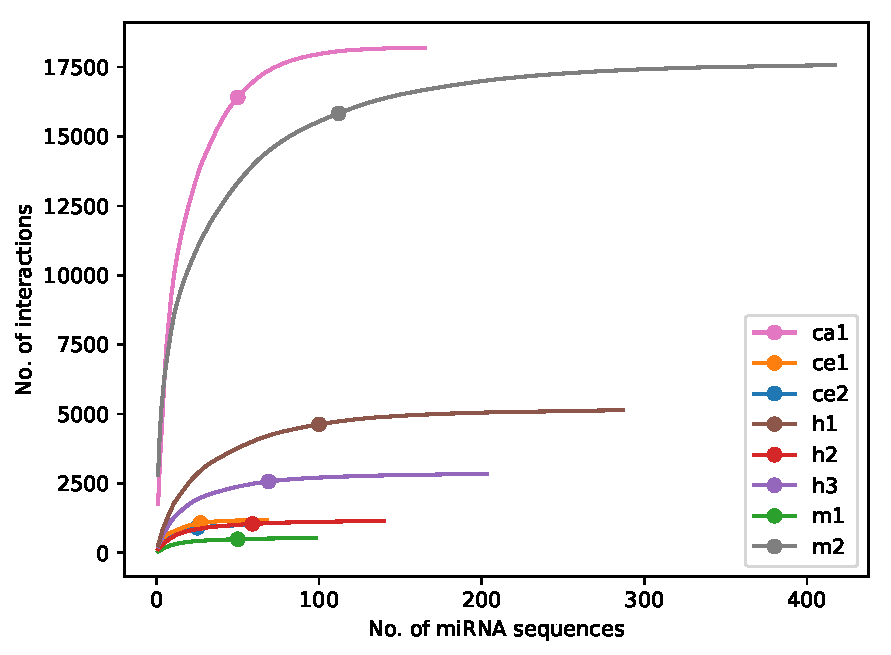
\includegraphics[width=0.6\textwidth]{images/1_mirna_dist.pdf}
      \label{fig:datasetplot}
 
      \end{figure}
\end{frame}

\begin{frame}{Classification of the miRNA-target duplexes}
\begin{figure}[h!]
  \caption{\textbf{Classification of the miRNA-target duplexes based on their base-pairing patterns}} 
    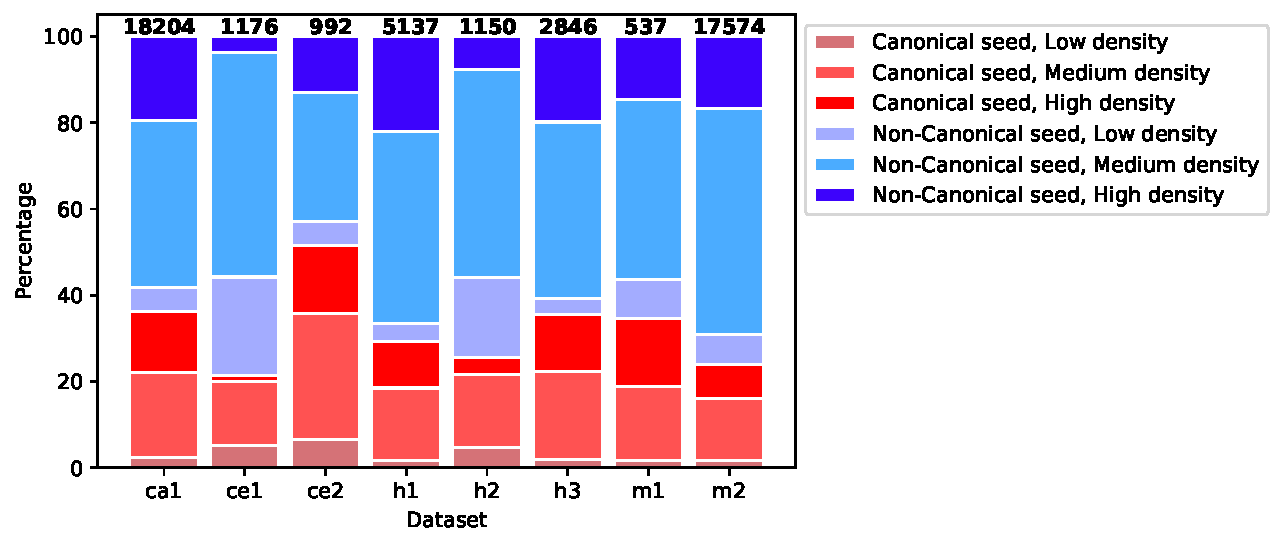
\includegraphics[width = 1\textwidth]{images/2_seed_type_positive2.pdf}
      \label{fig:seed_type_pos}
     
      \end{figure}
\end{frame}
      

\subsection{Intra-dataset analysis}
%%%%%%%%%%%%%%%%%%%%%%%%%%%%%%%%%%%%%%
\begin{frame}{Method}
\begin{itemize}
\item Feature extraction
\item Training/ testing split
\item Evaluation of different machine learning methods
\item In-depth analysis of the XGBoost performance
\item Top important features of each dataset
\end{itemize}
\end{frame}

\begin{frame}{Features}

\begin{table}[h!]
\label{tbl:feature_category}
 \resizebox{\textwidth}{!}{%
\begin{tabular}{|l|c|ll}
\hline
\textbf{Category}  & \multicolumn{1}{l|}{\textbf{No. of features}} & \multicolumn{1}{l|}{\textbf{Description}}                                                                                               & \multicolumn{1}{l|}{\textbf{Group}}              \\ \hline
Seed features      & 13                                        & \multicolumn{1}{l|}{Seed composition and properties}                                                                                    & \multicolumn{1}{l|}{High-level} \\ \hline
Free Energy        & 7                                         & \multicolumn{1}{l|}{\begin{tabular}[c]{@{}l@{}}Free energy of the duplex and the mRNA \\ at different regions\end{tabular}}                                                                    & \multicolumn{1}{l|}{High-level} \\ \hline
mRNA Composition   & 62                                        & \multicolumn{1}{l|}{mRNA composition in the site and flanking regions}                                                                           & \multicolumn{1}{l|}{High-level} \\ \hline
miRNA Pairing      & 38                                        & \multicolumn{1}{l|}{\begin{tabular}[c]{@{}l@{}}Binding information at each miRNA position \\ and across the miRNA-target duplex\end{tabular}} & \multicolumn{1}{l|}{Low-level}  \\ \hline
Site accessibility & 370                                       & \multicolumn{1}{l|}{Unpaired probabilities of each base}                                                                                                 & \multicolumn{1}{l|}{Low-level}  \\ \hline
Total              & 490                                       &                                                                                                                                         &                                                  \\ \cline{1-2}
\end{tabular}}
\end{table}
\end{frame}

\begin{frame}{Training/ testing split}
\begin{itemize}
\item Split ratio: 80\% training, 20\% testing
\item 20 sets of stratify splits
\begin{itemize}
\item Ensure that each miRNA appears in the training and the testing sets at the same proportion as in the original dataset.
\end{itemize}
\item 5 control sets (random split)
\end{itemize}
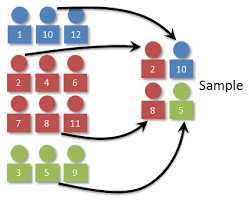
\includegraphics[width=0.5\textwidth,keepaspectratio]{images/stratify.png}
\end{frame}

\begin{frame}{Evaluation of different machine learning methods}
\begin{table}[h!]
\label{tab:self_summary}
   \resizebox{0.8\textwidth}{!}{%
\begin{tabular}{|l|l|l|l|l|l|l|}
\hline
Dataset & XGBoost & RF & KNN & SGD & SVM & LR \\ \hline
ca1                               & \begin{tabular}[c]{@{}l@{}}0.937 \\ (0.002)\end{tabular} & \begin{tabular}[c]{@{}l@{}}0.885 \\ (0.004)\end{tabular} & \begin{tabular}[c]{@{}l@{}}0.828 \\ (0.003)\end{tabular} & \begin{tabular}[c]{@{}l@{}}0.797 \\ (0.033)\end{tabular} & \begin{tabular}[c]{@{}l@{}}0.895 \\ (0.003)\end{tabular} & \begin{tabular}[c]{@{}l@{}}0.836 \\ (0.004)\end{tabular} \\ \hline
ce1                               & \begin{tabular}[c]{@{}l@{}}0.889 \\ (0.014)\end{tabular} & \begin{tabular}[c]{@{}l@{}}0.833 \\ (0.019)\end{tabular} & \begin{tabular}[c]{@{}l@{}}0.768 \\ (0.019)\end{tabular} & \begin{tabular}[c]{@{}l@{}}0.798 \\ (0.045)\end{tabular} & \begin{tabular}[c]{@{}l@{}}0.841 \\ (0.015)\end{tabular} & \begin{tabular}[c]{@{}l@{}}0.843 \\ (0.014)\end{tabular} \\ \hline
ce2                               & \begin{tabular}[c]{@{}l@{}}0.891 \\ (0.016)\end{tabular} & \begin{tabular}[c]{@{}l@{}}0.858 \\ (0.018)\end{tabular} & \begin{tabular}[c]{@{}l@{}}0.768 \\ (0.019)\end{tabular} & \begin{tabular}[c]{@{}l@{}}0.819 \\ (0.034)\end{tabular} & \begin{tabular}[c]{@{}l@{}}0.862 \\ (0.012)\end{tabular} & \begin{tabular}[c]{@{}l@{}}0.847 \\ (0.016)\end{tabular} \\ \hline
h1                                & \begin{tabular}[c]{@{}l@{}}0.824 \\ (0.007)\end{tabular} & \begin{tabular}[c]{@{}l@{}}0.769 \\ (0.008)\end{tabular} & \begin{tabular}[c]{@{}l@{}}0.731 \\ (0.007)\end{tabular} & \begin{tabular}[c]{@{}l@{}}0.746 \\ (0.011)\end{tabular} & \begin{tabular}[c]{@{}l@{}}0.795 \\ (0.007)\end{tabular} & \begin{tabular}[c]{@{}l@{}}0.770 \\ (0.007)\end{tabular} \\ \hline
h2                                & \begin{tabular}[c]{@{}l@{}}0.904 \\ (0.007)\end{tabular} & \begin{tabular}[c]{@{}l@{}}0.869 \\ (0.011)\end{tabular} & \begin{tabular}[c]{@{}l@{}}0.857 \\ (0.009)\end{tabular} & \begin{tabular}[c]{@{}l@{}}0.860 \\ (0.03)\end{tabular}  & \begin{tabular}[c]{@{}l@{}}0.879 \\ (0.009)\end{tabular} & \begin{tabular}[c]{@{}l@{}}0.892 \\ (0.009)\end{tabular} \\ \hline
h3                                & \begin{tabular}[c]{@{}l@{}}0.835 \\ (0.007)\end{tabular} & \begin{tabular}[c]{@{}l@{}}0.769 \\ (0.009)\end{tabular} & \begin{tabular}[c]{@{}l@{}}0.744 \\ (0.009)\end{tabular} & \begin{tabular}[c]{@{}l@{}}0.752 \\ (0.034)\end{tabular} & \begin{tabular}[c]{@{}l@{}}0.805 \\ (0.007)\end{tabular} & \begin{tabular}[c]{@{}l@{}}0.795 \\ (0.010)\end{tabular} \\ \hline
m1                                & \begin{tabular}[c]{@{}l@{}}0.847 \\ (0.015)\end{tabular} & \begin{tabular}[c]{@{}l@{}}0.795\\ (0.016)\end{tabular}  & \begin{tabular}[c]{@{}l@{}}0.758 \\ (0.022)\end{tabular} & \begin{tabular}[c]{@{}l@{}}0.760 \\ (0.038)\end{tabular} & \begin{tabular}[c]{@{}l@{}}0.819 \\ (0.019)\end{tabular} & \begin{tabular}[c]{@{}l@{}}0.800 \\ (0.019)\end{tabular} \\ \hline
m2                                & \begin{tabular}[c]{@{}l@{}}0.900 \\ (0.004)\end{tabular} & \begin{tabular}[c]{@{}l@{}}0.826 \\ (0.004)\end{tabular} & \begin{tabular}[c]{@{}l@{}}0.797 \\ (0.004)\end{tabular} & \begin{tabular}[c]{@{}l@{}}0.798 \\ (0.017)\end{tabular} & \begin{tabular}[c]{@{}l@{}}0.873\\ (0.004)\end{tabular}  & \begin{tabular}[c]{@{}l@{}}0.833 \\ (0.004)\end{tabular} \\ \hline
\end{tabular}}
\end{table}
\end{frame}



\begin{frame}{Top important features of each dataset}
   \begin{figure}[h!]
    \centering
      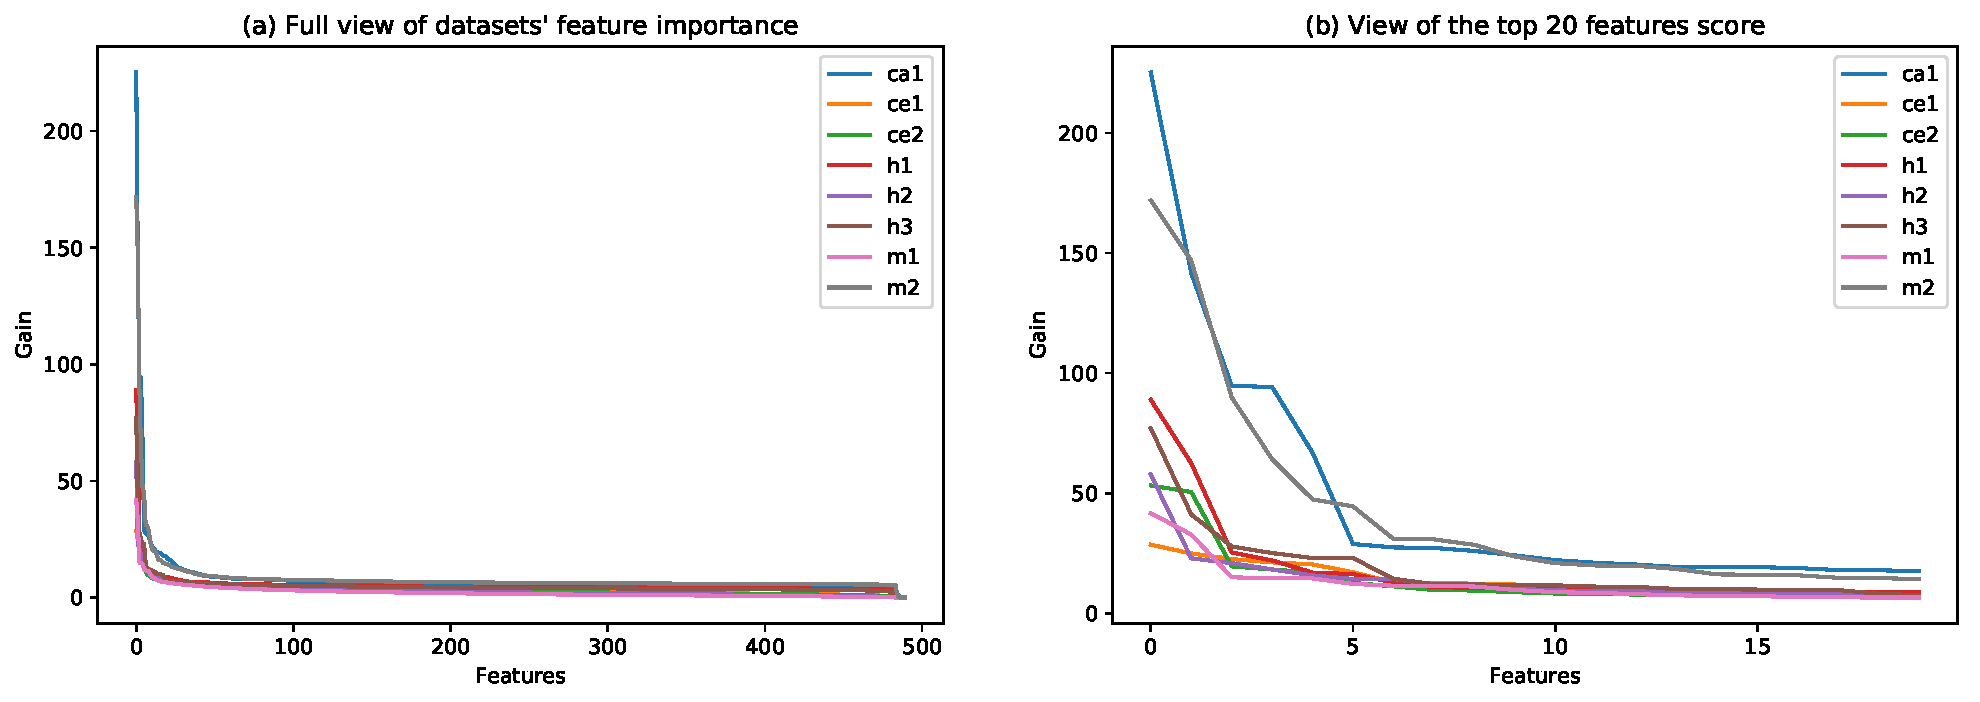
\includegraphics[width=\textwidth]{images/3_feature_importance.pdf}
      
    %   \caption*{The features are sorted in descending order from the top feature (highest gain) to lowest. (a) A full view of the gain plot emphasizes the gain decay.  (b) A zoomed view, focused on the top 20 features.}%
    
\end{figure}
\end{frame}



\begin{frame}{Top important features of each dataset}
\begin{table}[h!]
\caption{Feature importance}
\label{tab:feature_importance}
 \begin{threeparttable}
                     \resizebox{\textwidth}{!}{%

\begin{tabular}{|l|l|l|l|l|l|l|l|l|l|}
\hline
\textbf{Feature/Dataset}                          & \textbf{ca1} & \textbf{ce1} & \textbf{ce2} & \textbf{h1} & \textbf{h2} & \textbf{h3} & \textbf{m1} & \textbf{m2} & \textbf{mean} \\ \hline
\textbf{Number of GU bp within the seed\tnote{n}}              & 100\tnote{*}          & 87\tnote{*}           & 95\tnote{*}           & 29\tnote{*}          & 40\tnote{*}          & 100\tnote{*}         & 28          & 100\tnote{*}         & 72            \\ \hline
\textbf{bp in the 1st nt of the seed\tnote{b}}                    & 63\tnote{*}           & 79\tnote{*}           & 34\tnote{*}           & 70\tnote{*}          & 25\tnote{*}          & 30\tnote{*}          & 27          & 85\tnote{*}          & 52            \\ \hline
Number of GU bp within the site\tnote{n}                      & 42\tnote{*}           & 71\tnote{*}           & 32\tnote{*}           & 100\tnote{*}         & 19          & 53\tnote{*}          & 35\tnote{*}          & 28\tnote{*}          & 48            \\ \hline
Proportion of G in mRNA at the site region\tnote{n}                             & 12           & 74\tnote{*}           & 12           & 12          & 36\tnote{*}          & 33\tnote{*}          & 100\tnote{*}         & 37\tnote{*}          & 39            \\ \hline
Duplex minimum free energy\tnote{n}                               & 13\tnote{*}           & 45           & 11           & 10          & 100\tnote{*}         & 19          & 35\tnote{*}          & 52\tnote{*}          & 36            \\ \hline
\textbf{Number of bp at location 2-7\tnote{n}} & 42\tnote{*}           & 33           & 100\tnote{*}          & 12          & 18          & 36\tnote{*}          & 13          & 18          & 34            \\ \hline
Proportion of GG in mRNA at the site region\tnote{n}                            & 30\tnote{*}           & 21           & 10           & 12          & 7           & 30\tnote{*}          & 79\tnote{*}          & 26\tnote{*}          & 27            \\ \hline
\textbf{bp in the 4th nt of the seed\tnote{b}}                    & 8            & 100\tnote{*}          & 21           & 10          & 11          & 16          & 2           & 12          & 22            \\ \hline
Number of bulges outside the seed\tnote{n}                 & 3            & 60\tnote{*}           & 6            & 25\tnote{*}          & 32\tnote{*}          & 9           & 9           & 8           & 19            \\ \hline
\textbf{bp in the 2nd nt of the seed\tnote{b}}                    & 8            & 42           & 37\tnote{*}           & 7           & 11          & 13          & 15          & 6           & 17            \\ \hline
\textbf{bp in the 5th nt of the seed\tnote{b}}                    & 12           & 27           & 14           & 14          & 6           & 15          & 29\tnote{*}          & 12          & 16            \\ \hline
\textbf{Number of GC bp within the seed\tnote{n}}              & 7            & 22           & 24\tnote{*}           & 18\tnote{*}          & 12          & 13          & 11          & 12          & 15            \\ \hline
Number of GC bp outside the seed\tnote{n}                         & 4            & 27           & 11           & 10          & 27\tnote{*}          & 8           & 6           & 5           & 12            \\ \hline
Accessibility (nt=21, len=10)\tnote{n}                                    & 9            & 19           & 7            & 6           & 25          & 7           & 12          & 7           & 11            \\ \hline
minimum free energy of the target site + 50nt flanking regions\tnote{n}            & 8            & 11           & 6            & 7           & 8           & 11          & 36\tnote{*}          & 6           & 11            \\ \hline
\textbf{Number of mismatches inside the seed\tnote{n}}    & 4            & 3            & 15           & 19\tnote{*}          & 0           & 13          & 2           & 9           & 8             \\ \hline
\end{tabular}}

 \end{threeparttable}

\end{table}
\end{frame}

\subsection{Cross-dataset analysis}
\begin{frame}{Method}
Examine the relationships between datasets:
\begin{itemize}
\item Use a statistical measure to calculate the distance between the datasets. 
\item Visualize the datasets based on the unified list of the 16 most important features.
\item Evaluate the performance of each dataset specific classifier to properly classify interactions in the other datasets.
\end{itemize}
\end{frame}

\begin{frame}{Kullback Leibler divergence}
\begin{equation*}
 D_{KL} \left (P ||Q \right ) = \sum_{x\in \chi }{P\left ( x \right )log\left ( \frac{P\left ( x \right )}{Q\left ( x \right )} \right )}\label{eq:1}
\end{equation*}

   \begin{figure}[h!]
    \centering
      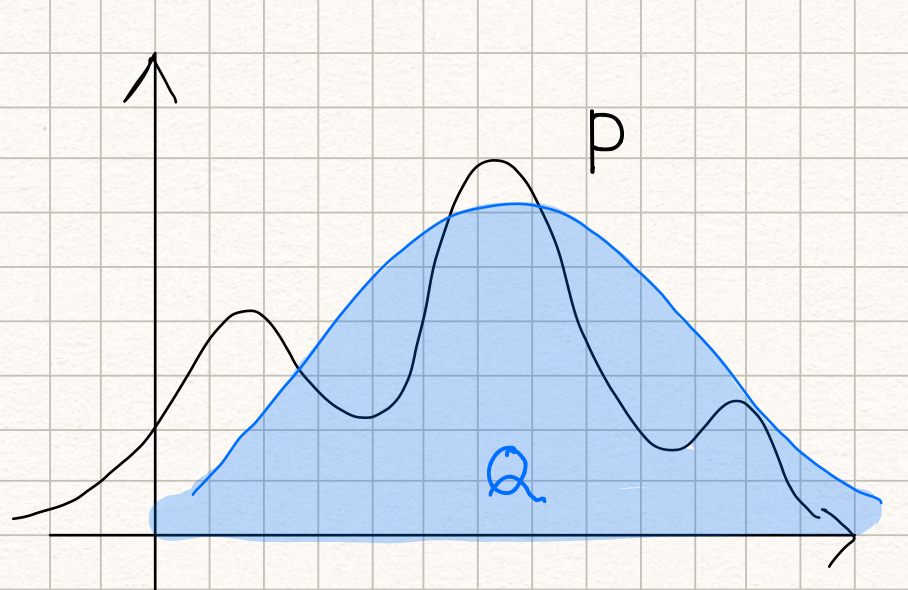
\includegraphics[width=0.8\textwidth]{images/kl_explain.png}
      \end{figure}

\end{frame}


\begin{frame}{Kullback Leibler divergence}
\begin{equation*}
 D_{KL} \left (P ||Q \right ) = \sum_{x\in \chi }{P\left ( x \right )log\left ( \frac{P\left ( x \right )}{Q\left ( x \right )} \right )}\label{eq:1}
\end{equation*}

  
\begin{itemize}
\item Measure the amount of information lost when the training set represents the testing set.
\item  \textit{P(x)} and \textit{Q(x)} are the \textbf{miRNA seed distribution functions}. 
\item \textit{Q(x)} is the approximation distribution (training set) 
\item \textit{P(x)} is the true distribution (testing set). 
\item The KL divergence is asymmetric.
\end{itemize}


\end{frame}



\begin{frame}{Kullback Leibler divergence}

\begin{figure}[h!]
      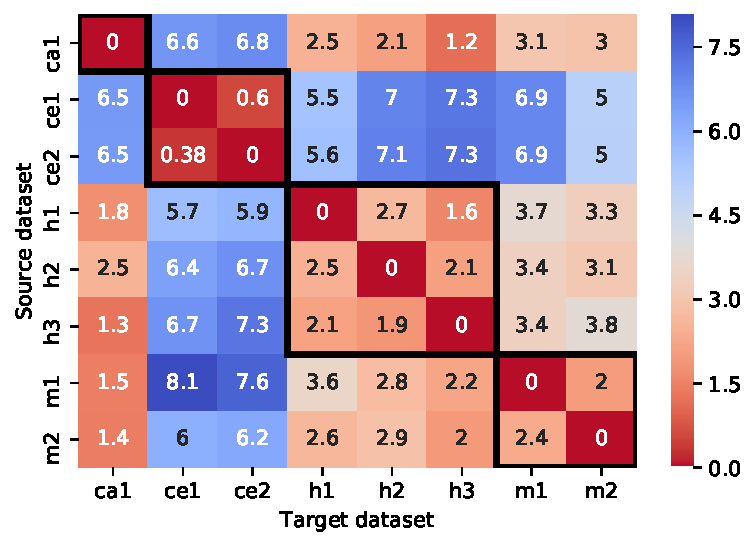
\includegraphics[width = 0.7\textwidth]{images/4_divergence_reverse.pdf}
      \label{fig:divergence}
      
      \end{figure}
\end{frame}

\begin{frame}{Dataset visualization using PCA}
\begin{figure}[h!]
  \caption{\textbf{Visualization of the datasets in 2D}} 
       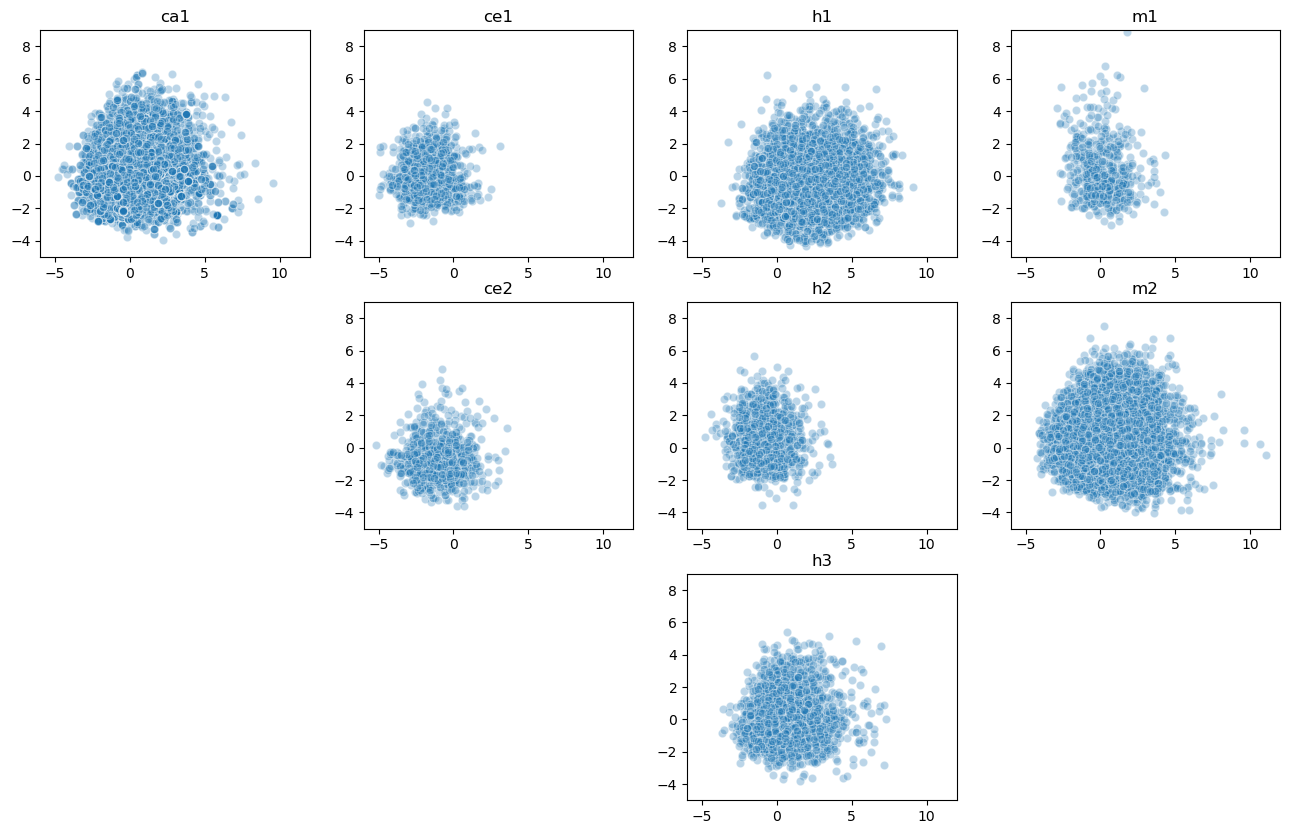
\includegraphics[width = 0.8\textwidth]{images/5_unite_features_pca_resample_scale=True_all.png}
      \label{fig:feature_pca}
      
      \end{figure}
\end{frame}

\begin{frame}{Classification performance between datasets}

\begin{figure}[h!]
      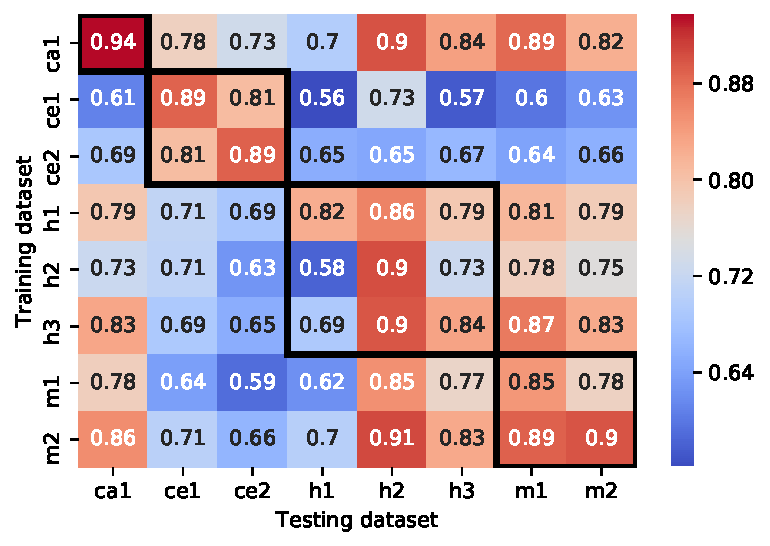
\includegraphics[width = 0.7\textwidth]{images/6_diff_summary.pdf}
    \label{fig:crossdataset}
    
      \end{figure}

\end{frame}

\section{Summary}
\subsection{Conclusions}
\begin{frame}{Methodology \& Results}

\begin{exampleblock}
		<1->{Methodology}
\begin{itemize}
\item Processing pipeline infrastructure
\item Thorough analysis of the datasets
\item Using tree-based classifier
\item Training and testing dataset split: stratify and control sets
\end{itemize}
\end{exampleblock}
\pause

\begin{exampleblock}
		<1->{Results}
\begin{itemize}
\item Cross-dataset accuarcy: 0.56 to 0.94. 
\item KL divergence - differences in miRNA distributions (different organisms, cell types...)
\item Area covered in 2D feature space - How the feature space is spanned by the datasets.
\end{itemize}


% \item Development of pipeline infrastructure enable us to analyze all available datasets.
% \item The importance of thorough analysis of the datasets
% \item Using tree-based classifier
% \item Training and testing dataset split: stratify and control sets
% \end{itemize}
\end{exampleblock}

\end{frame}




% \subsection{Methodology}
% \begin{frame}{Methodology}
% \begin{itemize}
% \item Development of pipeline infrastructure enable us to analyze all available datasets.
% \item The importance of thorough analysis of the datasets
% \item Using tree-based classifier
% \item Training and testing dataset split: stratify and control sets
% \end{itemize}
% \end{frame}

% \subsection{Results}
% % \begin{frame}{Evolutionary distance}
% % \begin{table}[h!]
% % \caption{Estimated divergence time {[}MYA{]} between organisms in our study}
% % \label{tab:evolutiontime}
% % \begin{tabular}{|l|l|l|l|}
% % \hline
% %              & Mouse & Cattle & C.elegans \\ \hline
% % Human & 90  & 96         & 797                    \\ \hline
% % Mouse          &     & 96         & 797                    \\ \hline
% % Cattle   &     &            & 797                    \\ \hline
% % \end{tabular}
% % \caption*{Each cell represents the time since the pair of organisms from the corresponding row and column diverged from their common ancestor (source: \cite{kumar2017timetree})}
% % \end{table}
% % \end{frame}


% \begin{frame}{Classification performance between organisms}
% \begin{itemize}
% \item The accuracy results of cross-dataset classification ranged between 0.56 to 0.94. 
% \item We examine several factors:
% \begin{enumerate}
% \item Evolutionary distance
% \begin{table}[h!]
% \label{tab:evolutiontime}
%                      \resizebox{0.5\textwidth}{!}{%
% \begin{tabular}{|l|l|l|l|}
% \hline
%              & Mouse & Cattle & C.elegans \\ \hline
% Human & 90  & 96         & 797                    \\ \hline
% Mouse          &     & 96         & 797                    \\ \hline
% Cattle   &     &            & 797                    \\ \hline
% \end{tabular}}
% \end{table}
% \item KL divergence - The divergence associates with the differences in miRNA distributions among different organisms, cell types or developmental stages.
% \item Area covered in 2D feature space - How the datasets spans the feature space.
% \end{enumerate}

 
% \end{itemize}
% \end{frame}



\begin{frame}{Conclusions}
\begin{exampleblock}
		<1->{Inter-organism prediction}
The accuracy is pretty high, as long as the organisms are within a certain evolutionary distance.
\end{exampleblock}
\pause
\begin{exampleblock}
		<1->{Universal interaction rules}
Machine learning model can generalize the interaction rules and learn the universal  rules. 
\end{exampleblock}
\pause

\begin{exampleblock}
		<1->{Transferability}
Target prediction models could be applied to organisms where experimental training data is limited or unavailable.
\end{exampleblock}

\end{frame}



% \begin{frame}{Conclusions}
% \begin{exampleblock}
% 		<1->{Conclusions}
% \begin{itemize}
% \item The accuracy are pretty high, as long as the organisms are within a certain evolutionary distance.
% \item Ability of the machine learning model to generalize interaction rules into more universal interaction rules. 
% \item Target prediction models could be applied also to organisms where experimental training data is limited or unavailable.
% \end{itemize}
% \end{exampleblock}

% \end{frame}
\subsection{Future work}
\begin{frame}{Future work}
\begin{itemize}
\item Add more miRNA-mRNA interaction datasets when become available.
\item Database and web server with parsed data, feature extraction and negative data.
\item Combine the information from several datasets and examine the prediction accuracy in close and more distant organisms.
\end{itemize}
\end{frame}

\section{MirTarFeaturesDB}
\subsection{Web server}
\begin{frame}{MirTarFeaturesDB}


\begin{figure}[h!]
  \caption{\textbf{search interaction window}}
      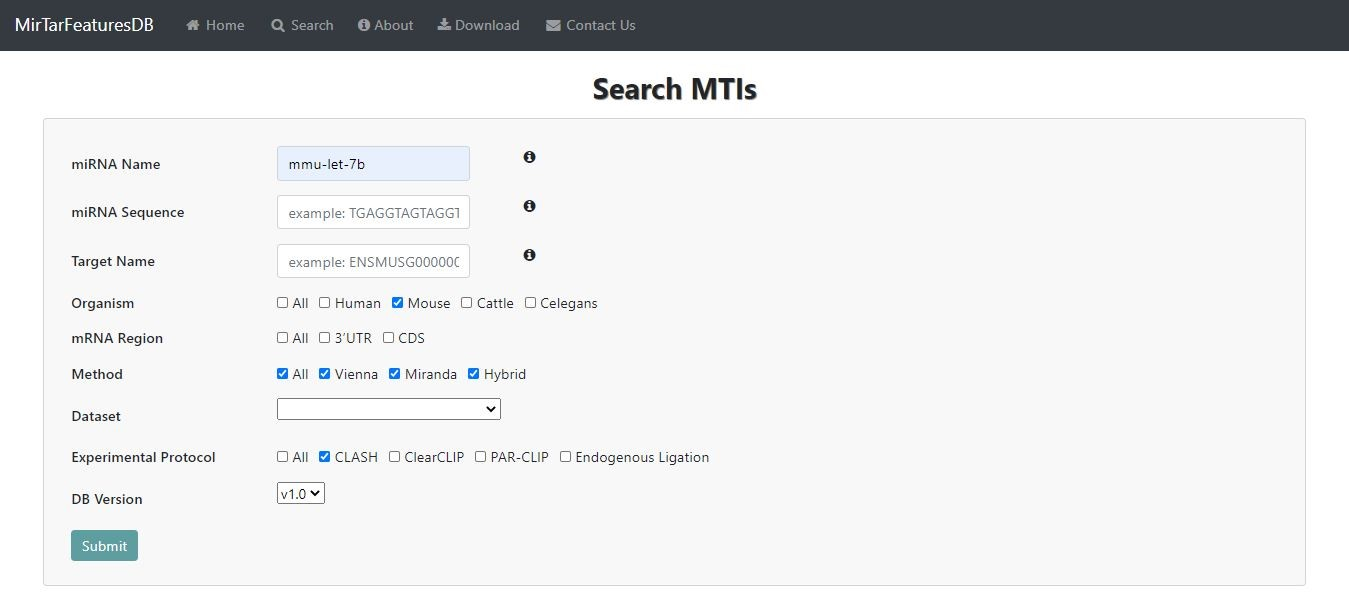
\includegraphics[width = 1\textwidth]{db figures/search interaction window.jpg}
      \label{fig:search}
          \end{figure}
\end{frame}
\begin{frame}{MirTarFeaturesDB}


\begin{figure}[h!]
  \caption{\textbf{Result window}}
      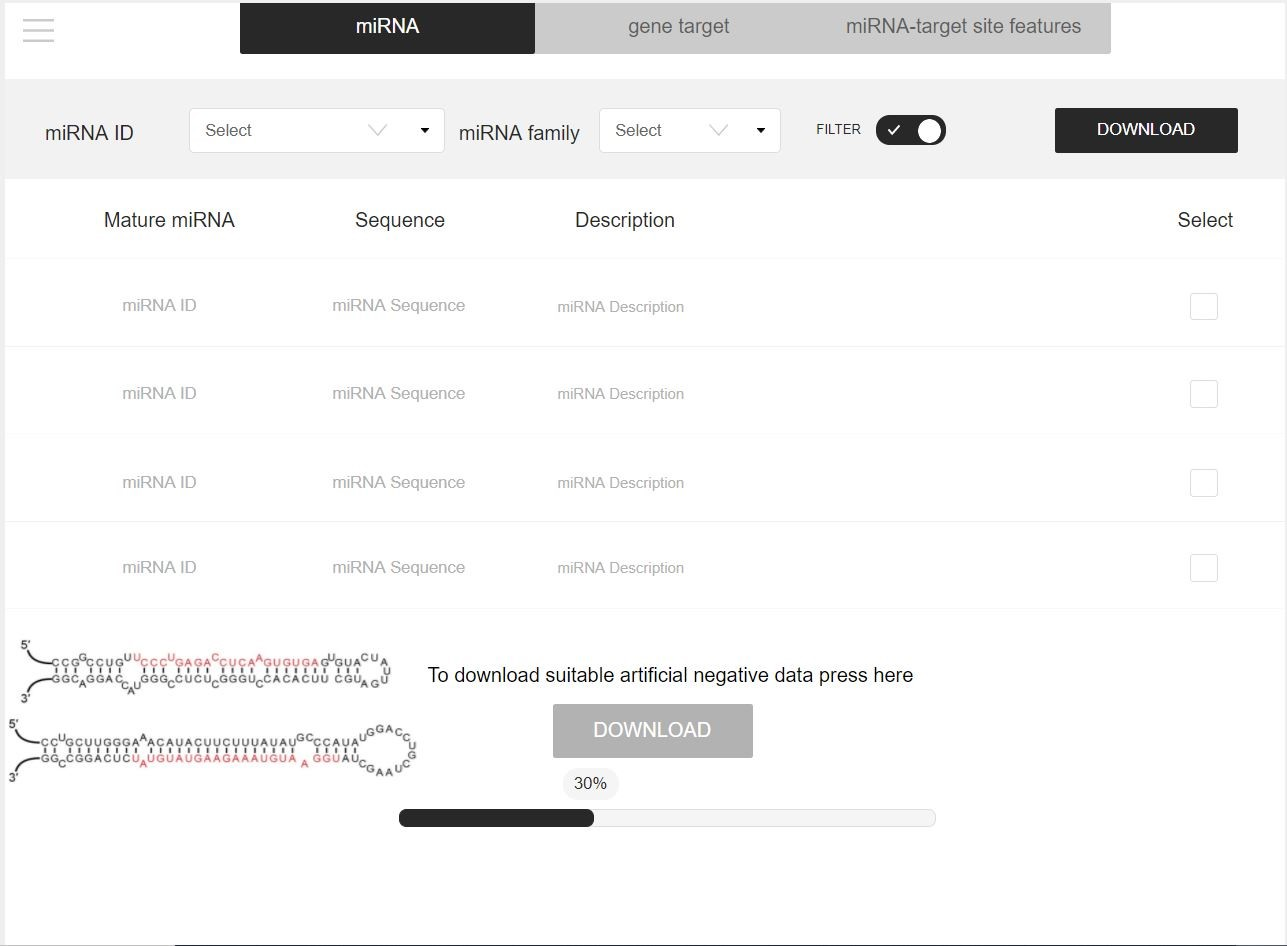
\includegraphics[width = 1\textwidth]{db figures/result.jpg}
      \label{fig:dbresult}
          \end{figure}
\end{frame}
\begin{frame}{MirTarFeaturesDB}



\begin{figure}[h!]
  \caption{\textbf{Download interaction file}}
      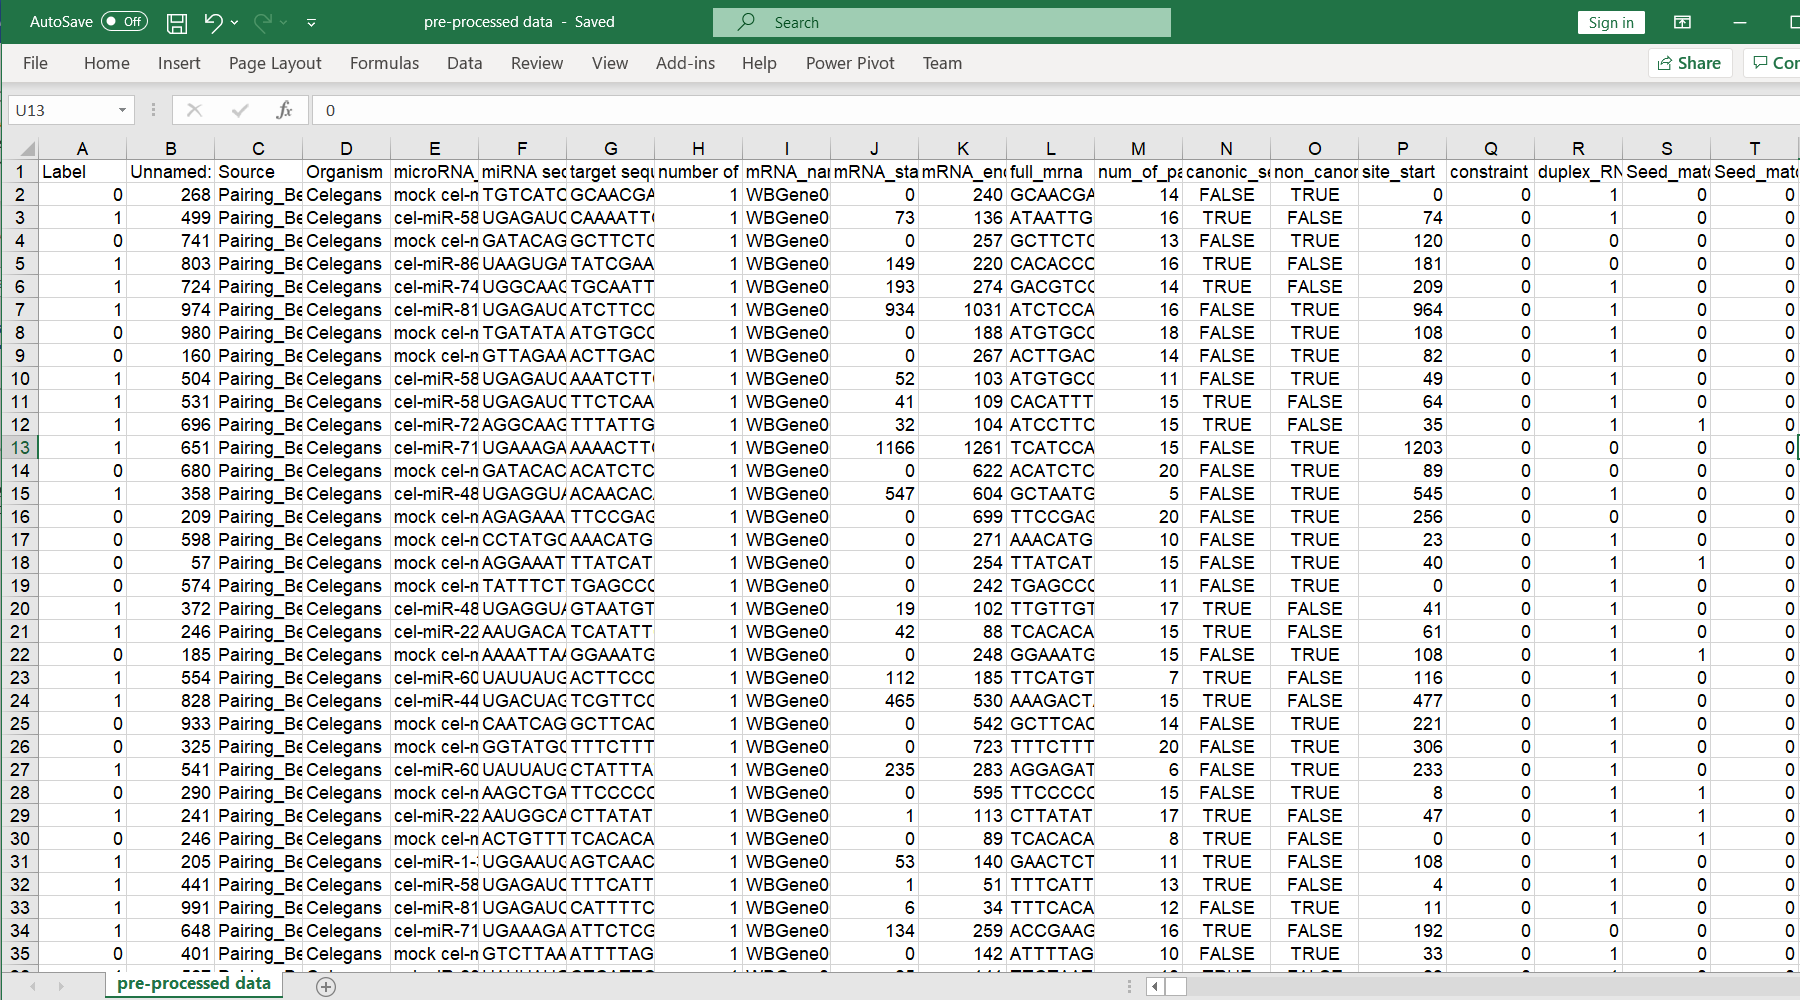
\includegraphics[width = 1\textwidth]{db figures/download.png}
      \label{fig:download}
          \end{figure}
\end{frame}


\end{document}